\documentclass{article}
\usepackage[utf8]{inputenc}
\usepackage{amsmath}
\usepackage{amsfonts}
\usepackage{tikz}

\begin{document}

\thispagestyle{empty}

\begin{figure}[htbp]
\centering
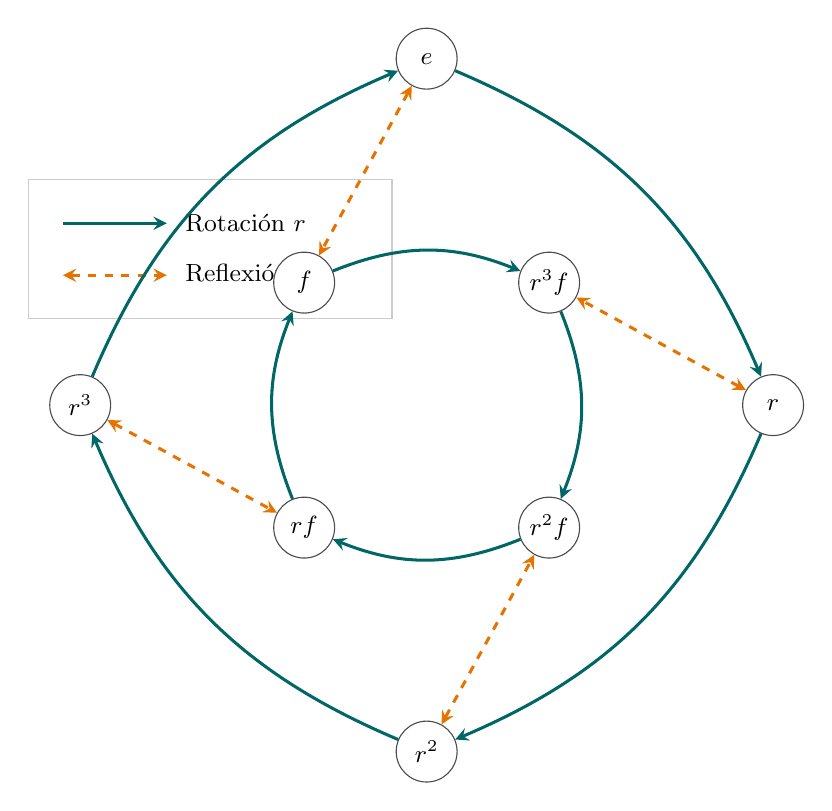
\begin{tikzpicture}[
    scale=2.2,
    % Estilo para los nodos
    nodo/.style={
        circle, 
        draw=black!70, 
        fill=white, 
        inner sep=1.5pt, 
        minimum size=2.2em, 
        font=\small
    },
    % Estilo para las rotaciones (flecha continua teal)
    flechaRotacion/.style={
        ->, 
        >=stealth, 
        thick, 
        color=teal!80!black, 
        line width=1.1pt
    },
    % Estilo para las reflexiones (flecha doble punteada naranja)
    flechaReflexion/.style={
        <->, 
        >=stealth, 
        thick, 
        color=orange!90!black, 
        dashed, 
        line width=1.1pt
    }
]

    % --- LEYENDA (Esquina superior izquierda) ---
    \begin{scope}[shift={(-2.3,1.3)}]
        \draw[draw=gray!40, fill=white] (0,0) rectangle (2.1,-0.8);
        \draw[flechaRotacion] (0.2,-0.25) -- (0.8,-0.25);
        \node[right, font=\small] at (0.85,-0.25) {Rotación $r$};
        
        \draw[flechaReflexion] (0.2,-0.55) -- (0.8,-0.55);
        \node[right, font=\small] at (0.85,-0.55) {Reflexión $f$};
    \end{scope}

    % --- VÉRTICES EXTERIORES (Direcciones Cardinales) ---
    \node[nodo] (e)  at (90:2.0)  {$e$};
    \node[nodo] (r)  at (0:2.0)   {$r$};
    \node[nodo] (r2) at (270:2.0) {$r^2$};
    \node[nodo] (r3) at (180:2.0) {$r^3$};

    % --- VÉRTICES INTERIORES (Direcciones Diagonales) ---
    \node[nodo] (f)   at (135:1.0) {$f$};
    \node[nodo] (r3f) at (45:1.0)  {$r^3 f$};
    \node[nodo] (r2f) at (315:1.0) {$r^2 f$};
    \node[nodo] (rf)  at (225:1.0) {$r f$};

    % --- CICLO DE ROTACIONES EXTERIORES (e -> r -> r^2 -> r^3 -> e) ---
    \draw[flechaRotacion] (e)  to[bend left=22] (r);
    \draw[flechaRotacion] (r)  to[bend left=22] (r2);
    \draw[flechaRotacion] (r2) to[bend left=22] (r3);
    \draw[flechaRotacion] (r3) to[bend left=22] (e);

    % --- CICLO DE ROTACIONES INTERIORES (f -> r^3f -> r^2f -> rf -> f) ---
    \draw[flechaRotacion] (f)   to[bend left=22] (r3f);
    \draw[flechaRotacion] (r3f) to[bend left=22] (r2f);
    \draw[flechaRotacion] (r2f) to[bend left=22] (rf);
    \draw[flechaRotacion] (rf)  to[bend left=22] (f);

    % --- ARISTAS DE REFLEXIÓN (Conexiones Naranja <->) ---
    \draw[flechaReflexion] (e)  -- (f);
    \draw[flechaReflexion] (r)  -- (r3f);
    \draw[flechaReflexion] (r2) -- (r2f);
    \draw[flechaReflexion] (r3) -- (rf);

\end{tikzpicture}
\end{figure}

\end{document}
